\documentclass[twocolumn]{article}
\usepackage[utf8]{inputenc}
\usepackage[top=1in]{geometry}
\usepackage{graphicx}
\usepackage{hyperref}
\usepackage{amsmath}
\input{sym}
\title{ECE 417/598: Homework 2}
\date{Due on Feb 4th, 2021, before class, 12:59 PM.}
\newtheorem{prob}{Problem}

\newcommand{\bx}{\bar{x}}
\newcommand{\by}{\bar{y}}
\newcommand{\bz}{\bar{z}}
\begin{document}

\maketitle
\section{Jan 26 Lecture}

\begin{prob}
  In class we proved the Rodrigues formula that converts from axis-angle
  representation $(\theta, \hat{\bfk})$, where $\theta$ is the angle of rotation
  and $\hat{\bfk}$ is the axis of rotation. Let $\bfK = [\hat{\bfk}]_{\times}$ be
  the cross product matrix of $\hat{\bfk}$. The corresponding rotation matrix is
  given by,
  \begin{align}
    R(\theta, \hat{\bfk}) = \bfI + \sin \theta \bfK + (1-cos \theta) \bfK^2.
  \end{align}

  A exponential of a square matrix $\bfM$ is defined as
  \begin{align}
    \exp(\bfM) = \sum_{n=0}^\infty \frac{1}{n!} \bfM^k = \bfI + \frac{1}{1!}\bfM + \frac{1}{2!}\bfM^2 + \dots
  \end{align}

  Recall the series expansion of $\sin \theta$, and $\cos \theta$,
  \begin{align}
    \sin \theta = \theta - \frac{\theta^3}{3!} + \frac{\theta^5}{5!} - \dots
    \\
    \cos \theta = 1 - \frac{\theta^2}{2!} + \frac{\theta^4}{3!} - \dots
  \end{align}
\end{prob}

  \begin{enumerate}
   \item First prove that $\bfK^3 = - \bfK$. (10 marks, 10 minutes)
   \item Using the expansion of $\sin\theta$ and $\cos\theta$, prove that
     $R(\theta, \hat{\bfk}) = \exp(\theta \bfK)$. (30 marks, 30 minutes)
  \end{enumerate}

\begin{prob}
  Write a pair of functions in C++ that converts rotation matrix from axis-angle
  representation and vice versa. Recall that
  \begin{align}
    R(\theta, \hat{\bfk}) = \bfI + \sin \theta \bfK + (1-cos \theta) \bfK^2.
  \end{align}
  and to get axis-angle back from a given rotation matrix
  \begin{align}
    R = \begin{bmatrix}
      r_{11} & r_{12} & r_{13} \\
      r_{21} & r_{22} & r_{23} \\
      r_{31} & r_{32} & r_{33}
      \end{bmatrix},
  \end{align}
  we have
  \begin{align}
    \theta &= \cos^{-1} \left(\frac{\text{tr}(R) - 1}{2}\right)
    \\
    \hat{\bfk} &= \frac{1}{2\sin\theta}\begin{bmatrix}
      r_{32} - r_{23} \\
      r_{13} - r_{31} \\
      r_{21} - r_{12}
      \end{bmatrix} \text{ if  } \theta \ne 0 \text{ or } \pi.
  \end{align}
 If $\theta = 0 \text{ or } \pi$, then
 \begin{align}
   \hat{\bfk} = \pm\begin{bmatrix}
    \sqrt{(r_{11} + 1)/2}\\
    \sqrt{(r_{22} + 1)/2}\\
    \sqrt{(r_{33} + 1)/2}
   \end{bmatrix}
   \end{align}
  
  (30 marks. Estimated time: 30 min)
  \label{prob:euler-to-rotmat}
\end{prob}


\section{Jan 31 Lecture}
\begin{prob}
  Coming soon
  % For the given robot write down the axis-angle rotation from joint to joint
  % assuming the joint angles to be  $\theta_1$, $\theta_2$, $\theta_3$ respectively.
  % \\
  % 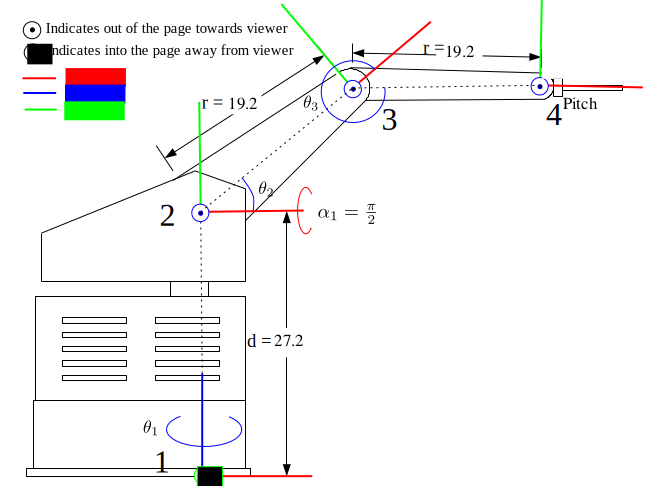
\includegraphics[width=\linewidth]{robot.png}
  % \\
\end{prob}

\section{ECE 598 only}

Write a short review of the following paper
\href{https://openaccess.thecvf.com/content_CVPR_2019/html/Zhou_On_the_Continuity_of_Rotation_Representations_in_Neural_Networks_CVPR_2019_paper.html}{On
  continuity of rotation representations in Neural networks}. We have not
covered all the concepts covered in this paper; you can skip the parts that you
do not understand. In the review answer the following questions evaluating the paper,
\begin{enumerate}
\item Problem: What problem is the paper trying to solve?
\item Approach: What is the proposed approach to solve the problem?
\item Contribution: What is the paper's novel contribution?
\item Evidence: Do they any experiments or proof that their approach/contributions work?
\item Results: Are the results of the paper justified by evidence and a direct
  result of the contibutions?
\end{enumerate}

%\bibliography{main}
%\bibliographystyle{plain}
\end{document}